\section{Protocolo In-Band}
\label{sec:ana_inband}

En esta sección, se tomará la decisión de seleccionar el protocolo de control in-band que se utilizará en el proyecto. Después de una cuidadosa evaluación de las opciones disponibles, se ha decidido utilizar el protocolo IoTorii \cite{rojas2021outperforming}, basado en el enfoque de enrutamiento jerárquico, como la solución más adecuada. Esta elección se respalda por el hecho de que el autor del proyecto ha participado activamente en el desarrollo del protocolo IoTorii, lo que garantiza un conocimiento profundo y una experiencia práctica en su implementación.\\
\\
El protocolo IoTorii ofrece una serie de ventajas significativas para el control in-band en entornos de \gls{iot}. Su enfoque jerárquico de etiquetado permite una gestión eficiente y escalable de la red, al tiempo que proporciona una mayor flexibilidad y adaptabilidad a las necesidades específicas del proyecto. Además, IoTorii ha sido probado y validado en diversas situaciones y escenarios, demostrando su eficacia y confiabilidad en la práctica.\\
\\
En este contexto, se ha tomado la decisión de hacer uso de los caminos generados por el protocolo IoTorii, donde cada nodo de la red posee rutas distintas para alcanzar el nodo raíz de la topología. En el caso de este proyecto, el nodo raíz se designará como el controlador (o el nodo que brinda acceso al controlador). Por lo tanto, la innovación radica en la implementación de IoTorii en un entorno de redes definidas por software (SDN).La integración de IoTorii con el entorno SDN permitirá aprovechar las capacidades y ventajas de ambos enfoques. La combinación de la eficiencia y escalabilidad jerárquica de IoTorii con la flexibilidad y el control centralizado de SDN ofrece un enfoque prometedor para el desarrollo y la gestión de redes \gls{iot}. Este enfoque innovador proporcionará una base sólida para llevar a cabo el proyecto y permitirá explorar nuevas posibilidades y mejoras en el ámbito del control in-band para entornos de \gls{iot}.

\subsection{Operativa del protocolo IoTorii}

\begin{figure}[ht!]
    \centering
    \includegraphics[width=\textwidth]{archivos/img/analisis/iotorii-operation.pdf}
    \caption{Operativa del protocolo de IoTorii \cite{rojas2021outperforming}}
    \label{fig:iotorii-operation}
\end{figure}

\begin{algorithm}[ht!]
    \SetAlgoLined
    %\KwResult{Write here the result }
    % initialization\;
    send \textit{Hello}\;
    \While{frame received}{
        %instructions\;
        \uIf{Hello}{
            \eIf{MAC not in Hello table}{
                assign unique \textit{suffix}\;
                save tuple \{\textit{MAC,suffix}\}\;
                \If{root node}{
                    create \textit{SetHLMAC} with HLMAC=1\;
                    \For{each tuple in Hello table}{
                        add tuple to \textit{SetHLMAC}\;
                    }
                    broadcast \textit{SetHLMAC}\;
                }
            }{
                discard\;
            }
        }
        \uElseIf{SetHLMAC}{
            \eIf{HLMAC (or prefix) not in HLMAC table}{
                save HLMAC in \textit{HLMAC table}\;
                create \textit{SetHLMAC} with received HLMAC\;
                \For{each tuple in Hello table}{
                    add tuple to \textit{SetHLMAC}\;
                }
                broadcast \textit{SetHLMAC}\;
            }{
                discard\;
            }
        }
        \Else{
            discard\;
        }
    }
    \caption{Assignment of HLMACs in IoTorii}
    \label{iotorii-alg}
\end{algorithm}

\begin{sidewaysfigure}
    \centering
    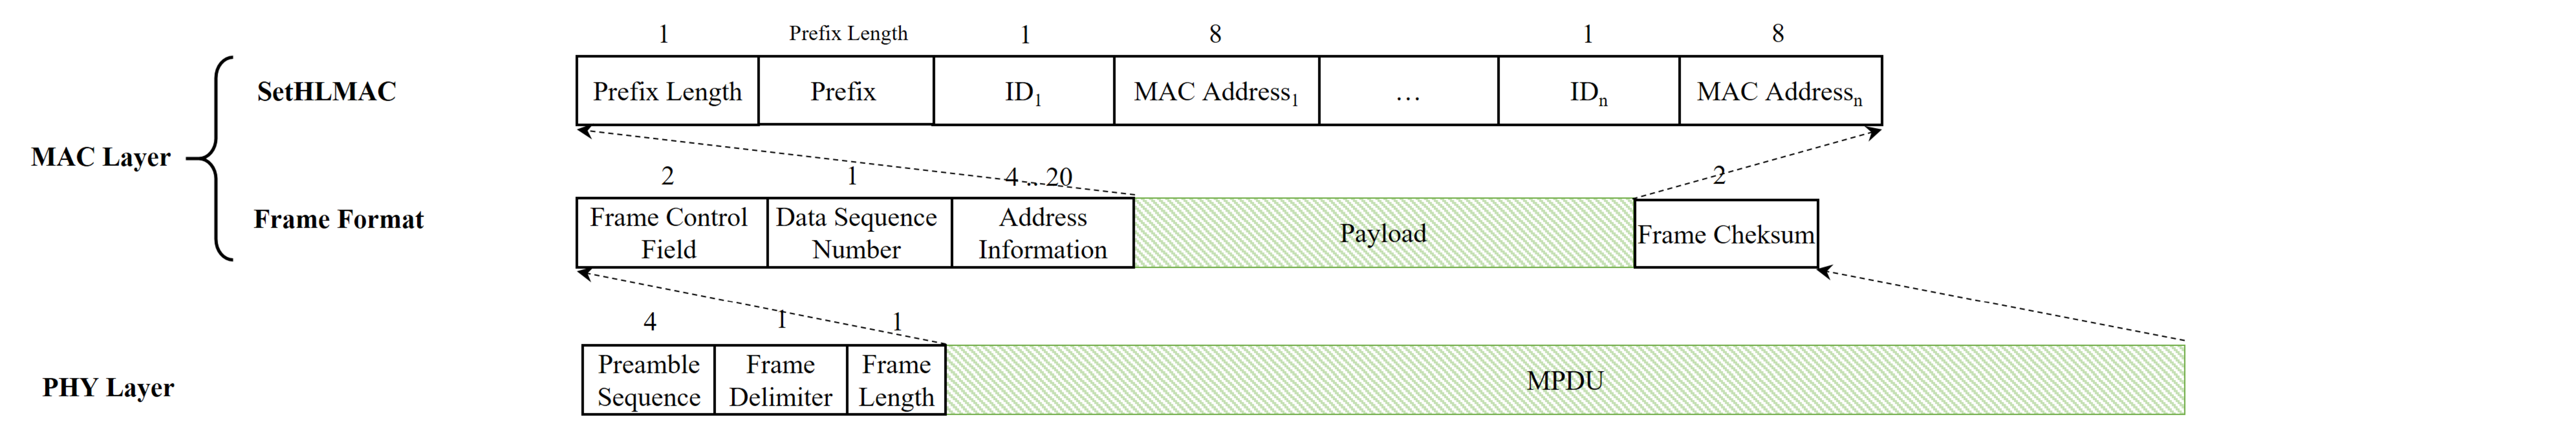
\includegraphics[width=\textwidth]{archivos/img/analisis/Comparation_frame_iotorii.eps}
    \caption{Mensajes de control en IoTorii \cite{rojas2021outperforming}}
    \label{fig:frameformat-setHLMAC}
\end{sidewaysfigure}


\subsection{Configuración del protocolo IoTorii}